% !TEX root = ../VPJ.tex

\chapter{Simulation}
\label{sec:Simulation}

Um verschiedene Programmabläufe und Funktionen zu testen war es wichtig, auch ohne realen Roboter die standardmäßige Programmfunktionalität darstellen zu können. Die Klasse SimulatedRobot erfüllt genau diese Anforderung. 

Mittels einer simulated-Flag kann in der Main-Funktion ein Simulationsbetrieb gestartet werden. In diesem ist kein realer Roboter notwendig, und trotzdem findet eine normale Auftragsplanung- und Abarbeitung statt. Die simulated-Flag wird in der Initialisierung dem UDP-Handler übergeben, der die Kommunikation mit den Robotern übernimmt. Somit wird in der Simulation kein Socket erzeugt und verbunden (siehe \ref{sec:UdpHandler}), sondern die Klasse SimulatedRobot genutzt. 

SimulatedRobot enthält eine State-Machine mit 13 Zuständen, die den Roboter ausreichend nachbilden. Weiterhin werden Funktionen für das simulierte Senden des Roboters an den UDPHandler und Timer für die Zustandswechsel bereitgestellt. 

Wie im echten Roboter wird der aktuelle Auftrag und Auftragstyp zwischengespeichert. 

\subsection{Zustandsdiagramm simulierter Roboter}

Das Zustandsdiagramm in Abbildung \ref{fig:simRobot} beschreibt die Zustände und Transitionen eines simulierten Roboters. Das Diagramm wurde anschließend als State Machine (vgl. \ref{sec:StateMachines}) implementiert. 

\begin{figure}[htb]
    \centering
    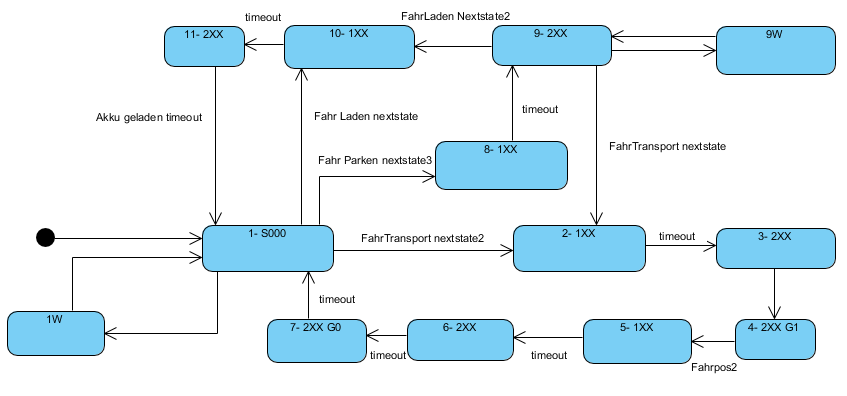
\includegraphics[width=0.9\textwidth]{Abbildungen/SimulatedRobot.PNG}
    \caption{Ablaufdiagramm des simulierten Roboters}		
    \label{fig:simRobot}
\end{figure}

Da in der Fertigungsplanung für die Vergabe der Aufträge die tatsächliche Position des Roboters nicht berücksichtigt wird, wird im simulierten Roboter ausschließlich die für die Planung benötigte Status- und Greiferinformation nachgepflegt. 

Die Änderung der Statusinformation ist im Diagramm in den Zuständen als Zahl mit zwei folgenden Dont-Care (XX) gekennzeichnet, da die Position keine weitere Relevanz hat. Eine Änderung des Greifers ist mit G0 für Greifer öffnet sich oder G1 für Greifer schließt sich gekennzeichnet.

Zur Initialisierung wurden ähnlich der State Machine aus Kapitel \ref{sec:StateMachineImplementierung} zunächst alle Zustände und Transitionen hinzugefügt, verknüpft und die State Machine gestartet. 

Der Initialzustand 1 kann über Empfang eines Auftrags zum Laden zu Zustand 10, zum Parken zu Zustand 8 oder zum Transport zu Zustand 2 verlassen werden. Außerdem wird das aktive Abfragen eines Auftrags an den Roboter alle 3 Sekunden über den Zustand 1W getriggert. Über den Wartezustand wird ein bearbeiteter noch anliegender Auftrag zurückgesetzt. 

Der Ablauf innerhalb der State-Machine zwischen zwei Aufträgen erfolgt über fest definierter Timer, die Zustandswechsel bewirken und ein Senden des Roboterstatus an den UDP-Handler hervorrufen.

Da innerhalb von QT keine Events verloren gehen kann auf ein periodisches Senden, wie der echte Roboter es tut verzichtet werden.

\subsubsection{Simulierte Ladefahrt}

Wenn in Zustand 1 am simulierten Roboter ein Ladefahrtauftrag anliegt, also ein Auftrag mit der ID 3, so wird direkt in Zustand 10 gewechselt. Es wird an den UDP-Handler ein Status 100 zurückgegeben  (auf dem Weg zur Ladestation) und ein Timer von 3 Sekunden gestartet. Nach Ablauf des Timers wird in Zustand 11 der Status 2XX zurückgegeben, was bedeutet, dass die Ladestation erreicht wurde. Nach Ablauf weiterer 5 Sekunden gilt das Laden als beendet und der Roboter geht in Zustand 1 über und sendet Status 000.

\subsubsection{Simulierter Parkvorgang}

Bei einem Parkauftrag in Zustand 1, also ein Auftrag mit der ID 2, wird in Zustand 8 gewechselt. An den UDP-Handler wird, da der simulierte Roboter jetzt auf dem Weg zum Parken ist, als Status 100 zurückgegeben. Nach einer Fahrzeit von 3 Sekunden hat der Roboter sein Ziel erreicht und gibt in Zustand 9 als Status 200 an den UDP-Handler. 

Zustand 9 kann entweder über einen Auftrag mit der ID 3 in Zustand 10 verlassen werden, und eine Ladefahrt wird simuliert, oder mit einem Auftrag und der ID 1 einen Transportauftrag in Zustand 2 verlassen werden. 

Über den Wartezustand 9W kann auf weitere Aufträge reagiert werden. Dieser wird alle 3 Sekunden aufgerufen. 

\subsubsection{Simulierter Transport}

Sobald ein simulierter Roboter in Zustand 2 kommt wird an den UDP-Handler der Status 100 übermittelt, da der Roboter sich auf dem Weg zur ersten Auftragsposition befindet. Nach 3 Sekunden wird in Zustand 3 der Status 2XX gesendet, da der Roboter an der ersten Position angekommen ist. Eine weitere Sekunde später wird das Werkstück gegriffen, was durch Senden des Greiferstatus 1 in Zustand 4 übermittelt wird. In Zustand 5 wird über Ablauf eines zweisekündigen Timers der Status 100 gesendet, da sich der Roboter auf dem Weg zur zweiten Station des Auftrags befindet. 

In Zustand 6, der nach 3 Sekunden bearbeitet wird, wird zunächst der Status auf 2XX gesetzt, da der Roboter angekommen ist. Nach einer Sekunde wird über Zustand 7 der Greifer geöffnet und der Greiferstatus auf 0 zurückgesetzt. Zwei Sekunden später wird wieder in Zustand 1 auf einen neuen Auftrag gewartet. 
